\chapter{Opis projektnog zadatka}

		Cilj ovog projekta stvoriti je korisničku web aplikaciju \textit{"MaketaShop"} koja služi za objavljivanje multimedijskog sadržaja o izrađenim maketama te njihovu prodaju.
		
		Primarne su funkcionalnosti aplikacije: 
		\begin{packed_item}
			
			\item  objava sadržaja na stranici
			\item  prodaja artikala
			\item  prenošenje zahtjeva od korisnika do administratora
			\item  pohrana podataka o korisnicima
			
		\end{packed_item}
		
		
		\underbar{Objavljivanje priča} o izrađenim maketama osnovna je funkcionalnost aplikacije. Priča se objavljuje kao multimedijski sadržaj. Vrste multimedijskog sadržaja između kojih se može birati su slike, video ili tekst ili pak neke kombinacije navedenih formata. Sustav omogućuje administratoru objavljivanje sadržaja dok ih registrirani korisnici mogu samo predlagati. Predložene priče administrator pregledava te mu se nudi opcija odobravanja objave priče. Već spomenuti registrirani korisnici, kao i oni neregistrirani, mogu komentirati objavljene sadržaje. Registriranim korisnicima se nudi opcija i označavanja priče ocjenama “sviđa mi se” ili “ne sviđa mi se”. Korisnici mogu samo vidjeti broj pozitivnih i negativnih ocjena za pojedinu priču.
		
		Na početnoj stranici aplikacije nalaze se mini prikazi svih već objavljenih priča (eng. \textit{thumbnails}). Klikom na pojedinu priču, može se pogledati puni tekst priče i/ili galerija slika i videa te se prikazuje prostor za komentare. Komentari registriranih korisnika prikazuju korisničko ime i profilnu sliku, dok su komentari neregistriranih korisnika objavljeni pod rezerviranim korisničkim imenom “Gost” i predefiniranom profilnom slikom. Administrator stranice ima ponuđenu opciju stvaranja priče, odabirom koje mu se nudi sučelje za sastavljanje priče. Registrirani korisnik u sandučiću ima ponuđenu opciju predlaganja priče ili predlaganja teme administratoru. Kada korisnik odabere opciju za slanje vlastite priče, pojavljuje mu se isto sučelje kao kad administrator sastavlja vlastitu priču. Ako korisnik odluči samo predložiti temu, nudi mu se drukčije sučelje u kojemu unosi samo kratki prijedlog za administratora. Administrator ima pretinac u koji mu stižu prijedlozi tema i gotove priče registriranih korisnika i tamo mu je ponuđena opcija odobriti ili odbiti pojedine priče te dati povratnu informaciju korisniku hoće li ili neće obraditi predloženu temu. Korisnici također imaju pretinac u kojem je vidljivo jesu li njihovi prijedlozi prihvaćeni ili odbijeni
		
		\underbar{Korisnici} imaju opciju registrirati se. \\Prilikom registracije korisnik unosi sljedeće podatke:
		\begin{packed_item}
			
			\item  ime
			\item  prezime
			\item  korisničko ime
			\item  email adresa
			\item  lozinka
			\item  adresa
			
		\end{packed_item}
		 Pritom su korisnički podaci zapamćeni u bazi podataka i koriste se svaki put kada korisnik želi kupovati ili komentirati. Na taj način korisnik ne mora svaki put ispočetka upisivati svoje podatke ako je već registriran. Prilikom registracije, korisniku je pridijeljena predefinirana slika koja je ista kao za neprijavljene korisnike. Korisnik također ima svoju stranicu profila koja je vidljiva svim drugim korisnicima. Početne su postavke namještene tako da su svi korisnički podaci javni (osim podataka o plaćanju poput broja kreditne kartice), no korisnik ima opciju na svojoj stranici profila mijenjati postavke privatnosti - može sakriti neke od svojih podataka. Jedini podaci koje korisnik ne može sakriti su korisničko ime i profilna slika. Korisnik na svojoj stranici profila može mijenjati svoju profilnu sliku.
		 
		 Administratoru je dostupan popis svih registriranih korisnika. Ukoliko se neki od korisnika počne neprimjereno ponašati, administrator ima opciju zabrane pristupa pojedinom korisniku na stranici profila. Zabrana pristupa stranici aktivna je sve do ručne ponovne dozvole pristupa. 
		
		\underbar{Web trgovina} također je sastavni dio aplikacije. U web trgovini izložene su standardne makete koje se prodaju. Na početnoj stranici web trgovine, nalaze se samo male sličice koje prikazuju makete (eng. \textit{thumbnails}). Korisnik klikom na pojedinu sličicu može pregledati opis. Svaka maketa unutar svog opisa sadrži specifikaciju (dimenzije i materijale). Kupcu u web trgovini za svaku se maketu nudi odabir različitih materijala. Taj odabir utječe na cijenu makete te je cijena prikazana tek kada korisnik odabere materijal. Administrator ima opciju unošenja standardnih maketa u web trgovinu. Pritom mu se za to otvara sučelje unutar kojeg može staviti slike makete, specifikacije te definirati cijenu makete za svaki od dostupnih materijala izrade i broj dostupnih maketa na skladištu. Nakon što je maketa napravljena, administrator može uređivati maketu. Klikom na gumb za uređivanje koji je vidljiv na detaljnom pregledu svake makete, administratoru se prikazuje sučelje u kojem može promijeniti sva svojstva makete, to jest ime, specifikacije, sliku te cijenu za svaki materijal i broj dostupnih maketa na skladištu.
		
		Jedna od pogodnosti koje se nude registriranim korisnicima naručivanje je maketa prema vlastitim idejama. U sandučiću postoji opcija koji vodi korisnika na formular. Korisnik ga popunjava i pritom prilaže svoj tekstualni opis makete uz navođenje dimenzija i željenog materijala za izradu makete. Tako popunjeni formular šalje se administratoru. Administrator pregledava zahtjev i u slučaju prihvaćanja zahtjeva, kreira cijenu za njega koju šalje natrag korisniku. Potom korisnik ima mogućnost odbijanja ili prihvaćanja te cijene. U slučaju prihvaćanja narudžbe, izrađena će maketa biti poslana na mjesto prebivališta korisnika koje je vezano uz njegov profil.
		
		Već spomenuta funkcionalnost web trgovine zahtijeva i mogućnost plaćanja putem interneta. Nakon odabira željenih proizvoda, pregleda i potvrde sadržaja košarice, korisnik ispunjava formular za plaćanje. Neregistrirani korisnici unose sve svoje osobne podatke u formular. Registrirani korisnici imaju već ispunjeni formular. Sustav pamti povijest svih transakcija te su one dostupne isključivo administratoru. Registrirani korisnik ima pristup popisu samo svojih transakcija.
		
		\underbar{Web aplikacije sa sličnim funkcionalnostima} kao ovaj projekt, dakako, već postoje na tržištu. Daleko najsličnije popularno programsko rješenje društvena je mreža Pinterest (\url{https://www.pinterest.com}). Tamo korisnici mogu dijeliti priče i dodavati slike vlastitih rukotvorina. Daljnja je sličnost oblik prikaza priča koji je prikazan na slici \ref{fig:pinterest}. Pinterest korisniku priče prikazuje u mreži te se klikom na priču ona uvećava i korisnik može detaljnije pročitati ili pogledati više slika, kao i u ovom projektu.
		
		\begin{figure}[H]
			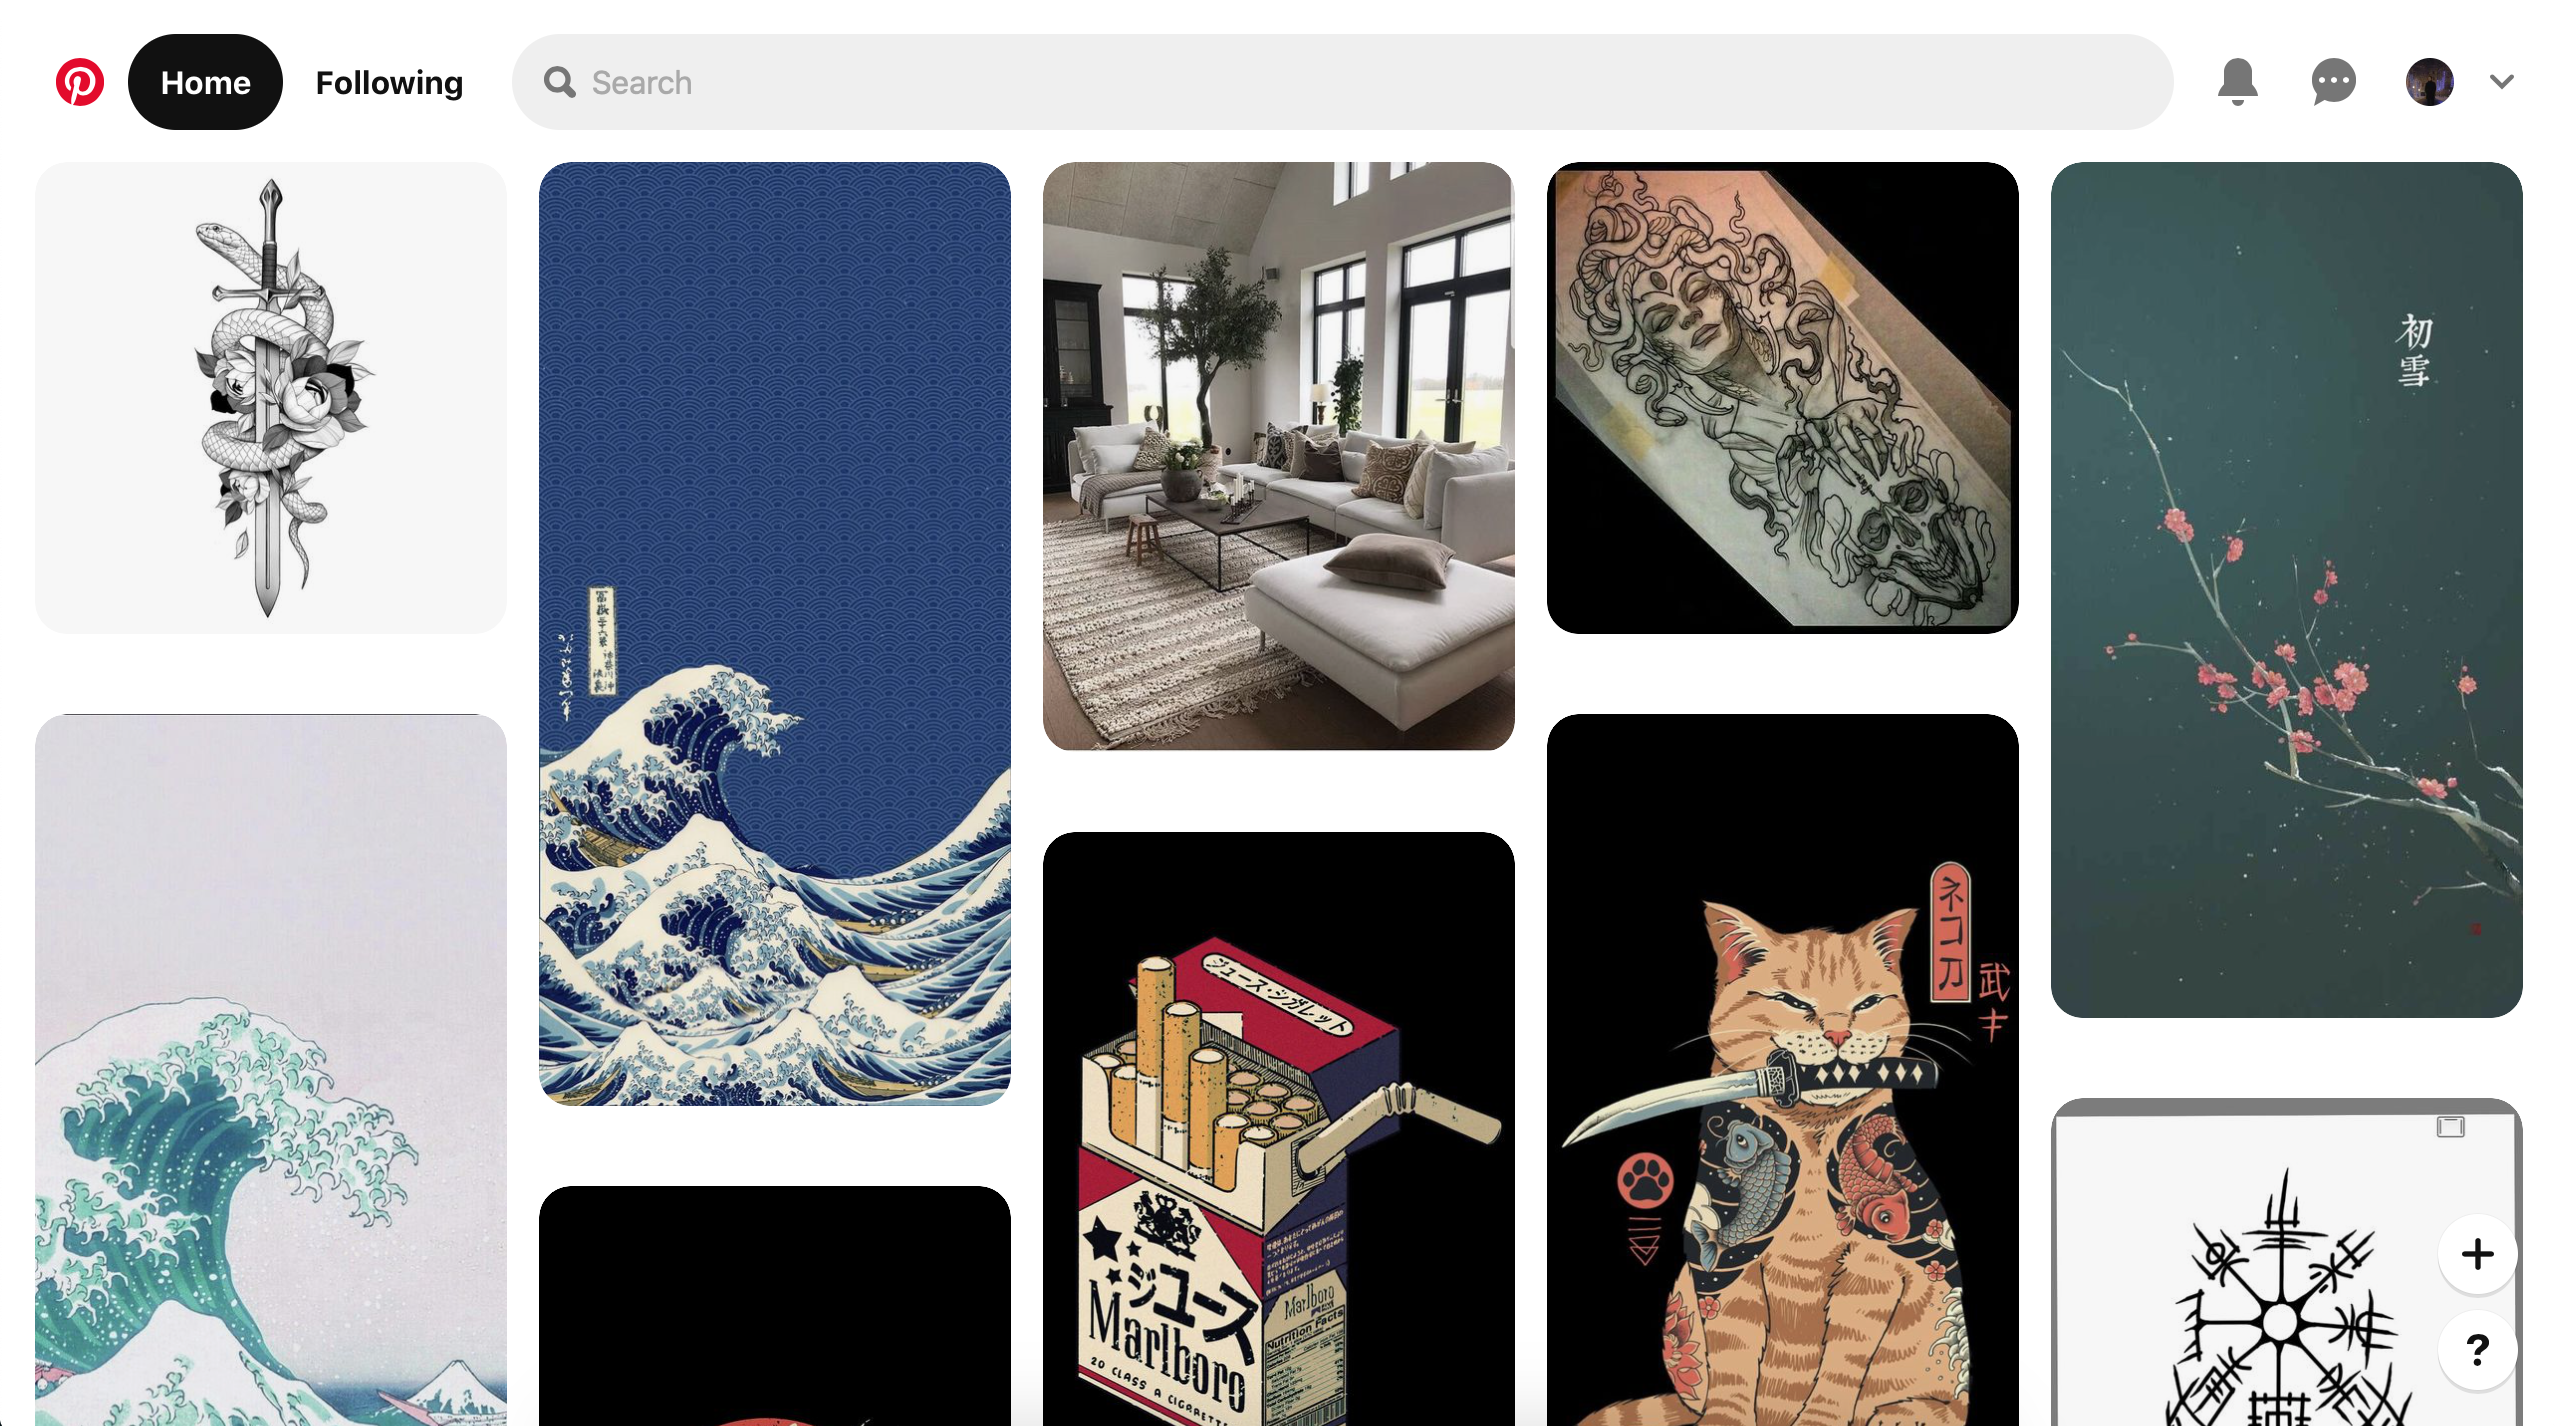
\includegraphics[scale=0.32]{slike/pinterest.PNG} %veličina slike u odnosu na originalnu datoteku i pozicija slike
			\centering
			\caption{Sučelje glavne stranice Pinteresta}
			\label{fig:pinterest}
		\end{figure}
	
		Društvena mreža Tumblr (\url{https://www.tumblr.com}) ima opciju isto takvog prikaza priča te ima slično sučelje za sastavljanje priča kakvo smo mi zamislili, prikazano na slici \ref{fig:tumblr}. Nadalje, Tumblr korisnicima nudi predlaganje tema ili postavljanje upita blogovima, slično kao što kod nas korisnici administratoru šalju prijedloge.
		
		\begin{figure}[H]
			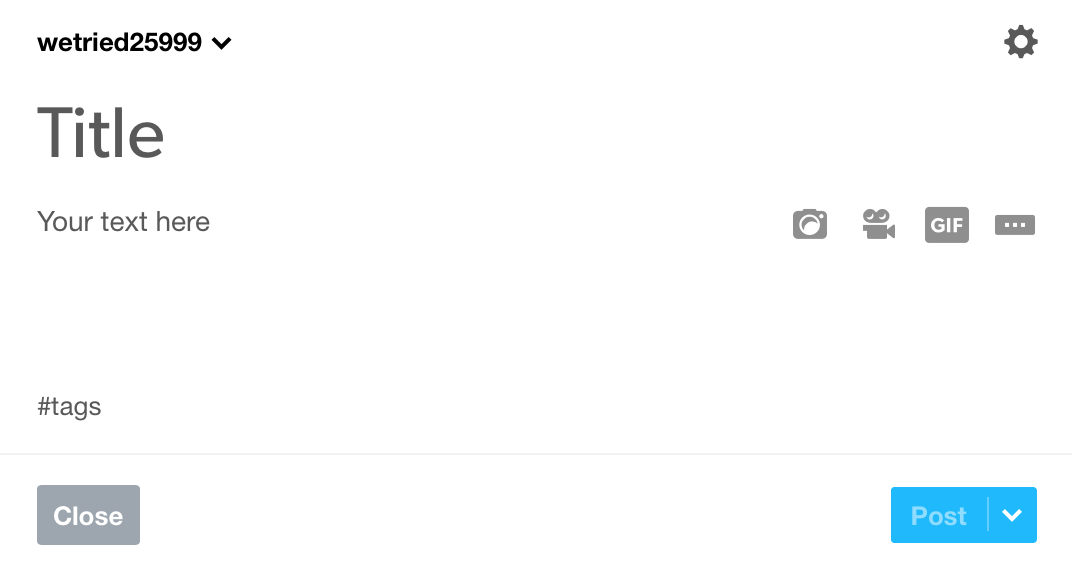
\includegraphics[scale=0.5]{slike/tumblr.PNG} %veličina slike u odnosu na originalnu datoteku i pozicija slike
			\centering
			\caption{Sučelje za sastavljanje priča na Tumblru}
			\label{fig:tumblr}
		\end{figure}
	
		Suštinska razlika tih dviju stranica i našeg projekta jest ta što su Pinterest i Tumblr primarno zamišljeni kao društvene mreže i kao takvi ne nude funkcionalnost web trgovine. Neke od popularnih usluga web trgovina koje su donekle slične našem rješenju su eBay, Njuškalo i Etsy. Što se tiče domene primjene, daleko je najsličniji Etsy (\url{https://www.etsy.com}), koji primarno služi za prodavanje proizvoda iz kućne radinosti i prodavačima pruža mogućnost postavljanja detaljnog opisa proizvoda, a kupcima komentiranje pojedinih proizvoda te postavljanje specifičnih zahtjeva prodavačima. Nasuprot tome, eBay i Njuškalo poprilično su standardne usluge web trgovine te se više fokusiraju na prodavanje proizvoda, a manje na komunikaciju među korisnicima te komunikaciju između kupca i prodavača.
		
		\underbar{Publika} na koju bismo ciljali s ovom specifičnom aplikacijom ne bi bila baš širokog spektra. Uglavnom bi se radilo o ljudima koji su entuzijastični oko izrade maketa ili kolekcionari. Mali bi prodavači maketa također mogli vidjeti korist u ovom sustavu s obzirom da bi imali još jednu platformu na kojoj mogu promovirati svoje proizvode.
		
		Ovakva aplikacija ima dosta usku i specifičnu primjenu te bi s vremenom sigurno zahtijevala nekakvo proširenje. Srodna bi ideja bila da se funkcionalnost proširi i na mogućnost objavljivanja raznih proizvoda iz kućne radinosti, a ne samo makete. To bi primjerice mogli biti razni ukrasi, mala kućna pomagala i slično. Generalizacijom domene primjene, aplikacija bi mogla obuhvatiti široku publiku. Primarno pri tome se misli na male poduzetnike i prodavače koji se žele osobno povezati sa svojom bazom kupaca i entuzijastima oko istih stvari.
		
		\underbar{Prilike za nadogradnju} ove aplikacije su mnogobrojne, no ovdje navodimo samo nekoliko ideja. Jedna od funkcionalnosti koja bi mogla biti nadogradnja na ovaj projektni zadatak bila bi mogućnost slanja poruka u stvarnom vremenu (eng. \textit{chat}) između registriranih korisnika i administratora te između samih korisnika. Još jedna nadogradnja na aplikaciju bilo bi daljnje personaliziranje profila. Registriranim bi korisnicima bile ponuđene dodatne opcije kao što su mijenjanje pozadinske slike aplikacije, promjena veličine, izgleda i boje slova i slično. Nadalje, administrator bi mogao objavljivati priče pod posebnim oznakama (eng. \textit{hashtag}) po kojima bi ih korisnici mogli pretraživati.

		\eject
		
	